\section{Lösen von Rekursionsgleichungen}
\begin{bsp}[note = Fibonacci-Folge , index = Fibonacci-Folge]
	\begin{gather*}
		f_n = f_{n-1} + f_{n-2} \qquad (n>1) \\
		f_0 = 0 \\
		f_1 = 1 \\
		\text{Explizite Darstellung } f_n = \dots \\
		\text{Ansatz: } f_n = \lambda^n \\
		\lambda^n = \lambda^{n-1} + \lambda^{n-2} \\
		( \lambda^2 - \lambda - 1 ) \lambda^{n-2} = 0 \qquad | \lambda \neq 0 \\
		\intertext{Charakteristisches Polynom}
		\lambda^2 - \lambda + 1 = 0 \\
		\lambda_{1,2} = \frac{1 \pm \sqrt{1+4}}{2} = \frac{1 \pm \sqrt{5}}{2} \\
		\text{Zwei Lösungen: } \lambda_1^n , \lambda_2^n . \\
		f_{a,b}(n) = a \cdot \lambda_1^n + b \cdot \lambda_2^n \\
		\text{Beh.: } f_{a,b}(n) \text{ ist die Lösung der Rekursion} \\
		\begin{split}
		f_{a,b}(n)	&= a \cdot \lambda_1^n + b \cdot \lambda_2^n \\
				&= a ( \lambda_1^{n-1} + \lambda_1^{n-2} ) + b ( \lambda_2^{n-1} + \lambda_2^{n-2} )	\\
				&= a \lambda_1^{n-1} + b \lambda_2^{n-1} + a \lambda_1^{n-2} + \lambda_2^{n-2} \\
				&= f_{a,b}(n-1) + f_{a,b}(n-2)
		\end{split}
		\intertext{Bestimmung von $a,b$ mit Randbedingungen}
		0 = a \underbrace{\left( \frac{1+\sqrt{5}}{2} \right)^0}_1 + b  \underbrace{\left( \frac{1-\sqrt{5}}{2} \right)^0}_1 \implies a = -b \\
		1 = (-b) \left( \frac{1+\sqrt{5}}{2} \right)^1 + b \left(  \frac{1-\sqrt{5}}{2} \right)^1 \\
		1 = -b \sqrt{5} \\
		b = -\frac{1}{\sqrt{5}} , a = \frac{1}{\sqrt{5}} , f_n = \frac{1}{\sqrt{5}} \left( \left( \frac{1+\sqrt{5}}{2} \right)^n - \left( \frac{1-\sqrt{5}}{2} \right)^n \right) \\
		|\lambda_2| < 1 \\
		f_n \approx \frac{1}{\sqrt{5}} \left( \underbrace{\frac{1+\sqrt{5}}{2}}_\lambda \right)^n \\
		\lambda \text{ ist Lösung von } \lambda^2 - \lambda +1 = 0 \\
		\lambda^2 = \lambda + 1 \\
		\frac{\lambda}{1} = \frac{\lambda + 1}{\lambda} \qquad \textbf{Goldener Schnitt}\index{goldener Schnitt}
	\end{gather*}
\end{bsp}
\todo{Too long}
\begin{bsp}
	\begin{gather*}
		g_n = 6 g_{n-1} - 12 g_{n-2} + 8 g_{n-3} \\
		g_0 = 1 \\
		g_1 = 2 \\
		g_2 = 3 \\
		\underbrace{\lambda^3 - 6 \lambda^2 + 12 \lambda - 8}_{=(\lambda-2)^3} = 0 \\
		\text{Lösungen: } 2^n , n \cdot 2^n , n^2 \cdot 2^n \\
		\intertext{Verifikation:}
		n \cdot 2^n \overset{?}{=} 6 (n-1) 2^{n-1} - 12 (n-2) 2^{n-2} + 8 (n-3) 2^{n-3} \\
		n \cdot 8 \overset{?}{=} 6(n-1)4 - 12(n-2)2 + 8(n-3) \\
		8n \overset{?}{=} 24n - 24 -24n +48 +8n -24 \quad \checkmark \\
		\intertext{Allgemeine Lösung:}
		g_n = a \cdot 2^n + b \cdot n \cdot 2^n + c \cdot n^2 \cdot 2^n \\
		\intertext{Sepezielle Lösung:}
		1 = a \\
		2 = 2a + 2b + 2c  \implies b = -c \\
		3 = 4a + 8b + 16c \implies 3 = 4+ 8c \\
		c = -\frac{1}{8} , b = \frac{1}{8} \\
		g_n = 2^n + \left( \frac{n - n^2}{8} \right) \cdot 2^n
	\end{gather*}
\end{bsp}
\begin{bsp}
	\begin{gather*}
	\underbrace{\overbrace{\Box}^{\frac{n}{2}} \overbrace{\Box}^{\frac{n}{2}}}_n * \underbrace{\overbrace{\Box}^{\frac{n}{2}} \overbrace{\Box}^{\frac{n}{2}}}_n \qquad \text{Divide et impera} \\
	T(n) = 4 \cdot T\left(\frac{n}{2}\right) \\
	T(1) = t_0\\
	\text{Substitution: } n =2^m \qquad m = \log_2 n \\
	T(2^m) = 4 \cdot T(2^{m-1}) \\
	S(m) = 4 \cdot S(m-1) \\
	\intertext{Löse $S$}
	\text{Char. Pol.: } \lambda - 4 = 0 \\
	\text{Allg. Lösung: } S(m) = a \cdot 4^m \\
	T(n) = S(\overbrace{\log_2 n}^m) = a \cdot 4^{\log_2 n} = a \cdot n^2 \\
	\text{Spez. Lösung: } T(n) = t_0 \cdot n^2
	\end{gather*}
\end{bsp}
$\Bigg[$Karatsuba\index{Karatsuba}: Es braucht nur 3 Mult.
\begin{gather*}
	T(n) = 3 \cdot T\left(\frac{n}{2}\right) \\
	\text{Ansatz: } T(n) = n^x \\
	\text{Einsetzen: } n^x = 3\left(\frac{n}{2}\right)^x \implies 3 =2^x \implies x = \log_2 3 \quad (<2) \\
	a \cdot b = a_1 b_1 K^2 + \underbrace{a_1 b_2 K + a_2 b_1 K}_{\underbrace{(a_1 b_2 + a_2 b_1)}_{\substack{(a_1 + a_2)(b_1 + b_2)\\ = a_1 b_1 + (a_1 b_2 + a_2 b_1) + a_2 b_2}}K} + a_2 b_2
\end{gather*}
Dimension\index{Dimension}:
\begin{gather*}
	\begin{matrix*}[l]
		\text{dim } 1:	&V(l) = l	\\
		\text{dim } 2:	&V(l) = l^2	\\
		\text{dim } 3:	&V(l) = l^3	
	\end{matrix*}\\
	V(l) = 4 V\left(\frac{l}{3}\right) \\
	l^d = 4 \cdot \left(\frac{l}{3} \right)^d \\
	3^d = 4 \\
	d = \log_3 4
\end{gather*}
$\Bigg]$\\
\begin{bsp}
	\begin{gather*}
		h(0) = 0 \\
		h(1) = 2 \\
		h(n) = 2h(n-1) - 2h(n-2) \\
		\text{Char. Pol.: } \lambda^2 - 2\lambda + 2 = 0 \\
		\lambda_{1,2} = \frac{2 \pm \sqrt{4-8}}{2} = 1 \pm i \\
		\text{Allg. Lös.: } a(1+i)^n + b(1-i)^n \\
		\text{Spez. Lös.: } 0 = a(1+i)^0 + b(1-i)^0 \implies b = -a \\
		2 = a(1+i) + (-a)(1-i) = 2ai \implies a = \frac{1}{i} = -i \\
		h(n) = \frac{1}{i} [(1+i)^n - (1-i)^n] \in \mathbb{N}
	\end{gather*}
\end{bsp}
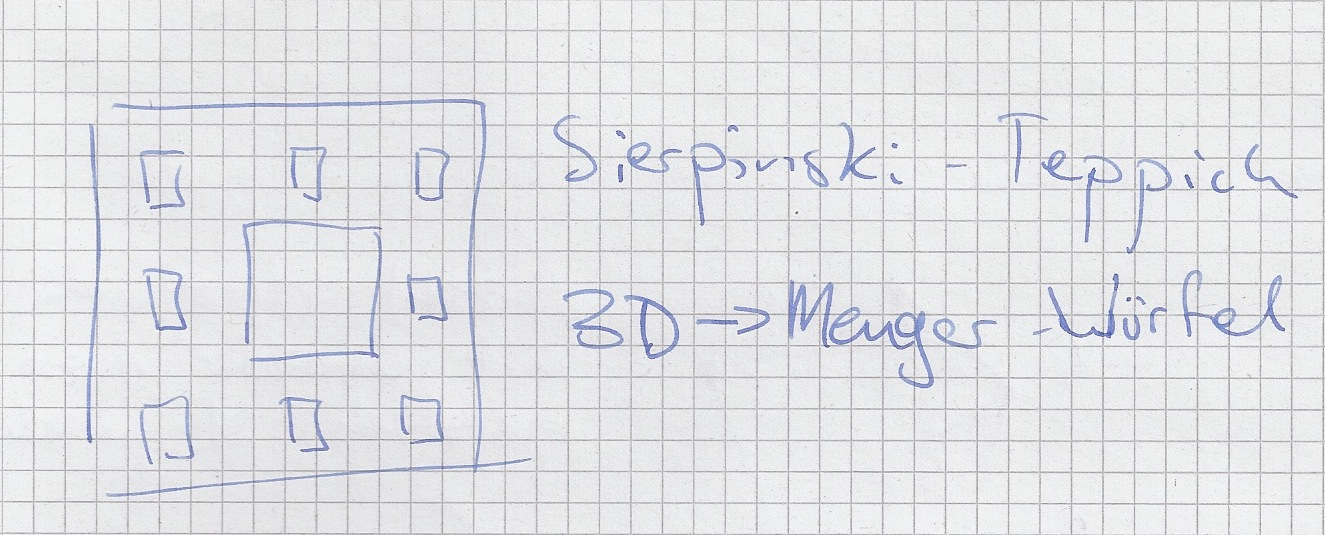
\includegraphics{Bild26} \\
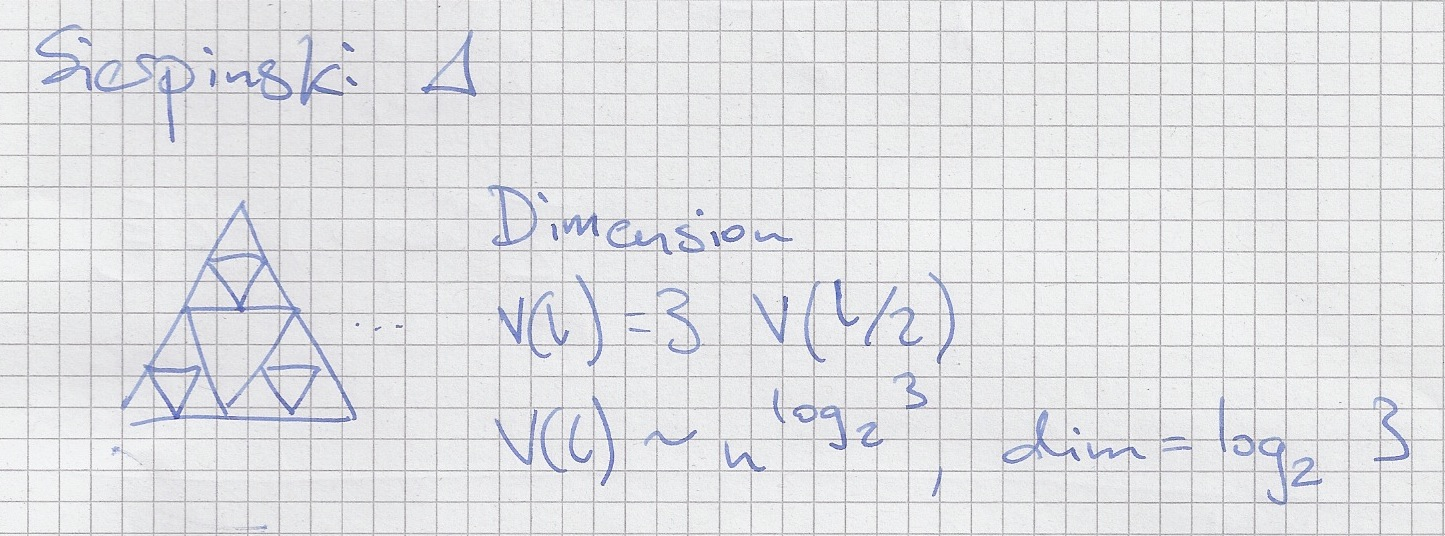
\includegraphics{Bild27}